\documentclass[../book-template.tex]{subfiles}

\begin{document}

\chapter{Principal Component Analysis}
In the last chapter, we discussed linear dimension reduction via linear autoencoder. Now we try to understand linear dimension reduction in a principled manner. We start with 1-dimension case, i.e. we want to approximate a group of points via points on a line. Then we generalize it to multiple dimensions, which yields exactly the idea of PCA. Finally we introduce a simple algorithm to find the dominant eigenvector of a matrix, followed by some examples and comparison with Linear Autoencoder we discussed in the last chapter.
\section{1D Linear Case}
\subsection{Line in \texorpdfstring{$\mathbb{R}^m$}{Rm}}
Mathematically, we can represent a line in $\mathbb{R}^m$ in the following parametric form:
\begin{equation*}
    \bm{\mu} + \mathbb{R}\bm{u} \equiv \{\bm{v}\in \mathbb{R}^m:\exists z\in \mathbb{R}\ s.t.\ \bm{v}=\bm{\mu} + z\bm{u} \}
\end{equation*}
where $\bm{\mu}$ is the offset or shift, $\bm{u}$ is the direction vector such that $\|\bm{u}\|=1$. Note that representation is not unique since a scaling on $\bm{u}$ and a shifting on $\bm{\mu}$ along $\bm{u}$ will not change the line. 
\subsection{Approximation of a single point: orthogonal projection}
Now consider the task to approximate a data point $\bm{x}\in\mathbb{R}^m$ by a point on the line. It natural to request that our approximation should be close to the original point in Euclidean distance. Formally, we try to solve
\begin{equation}\label{eq_2_1}
    \mathop{\arg\min}_{z\in\mathbb{R}}\|\bm{\mu}+z\bm{u}-\bm{x}\|^2
\end{equation}
or equivalently,
\begin{equation*}
    \mathop{\arg\min}_{\hat{\bm{x}}\in \bm{\mu} + \mathbb{R}\bm{u}}\|\hat{\bm{x}}-\bm{x}\|^2
\end{equation*}
To solve (\ref{eq_2_1}), we request the first order optimality condition:
\begin{equation*}
    \frac{d}{dz}\|\bm{\mu}+z\bm{u}-\bm{x}\|^2 = 2\langle \bm{\mu}+z\bm{u}-\bm{x}, \bm{u}\rangle \overset{!}{=}0
\end{equation*}
this yields solutions
\begin{align*}
    z &= \langle \bm{x}-\bm{\mu},\bm{u} \rangle\\
    \hat{\bm{x}} &= \bm{\mu} + \langle \bm{x}-\bm{\mu},\bm{u} \rangle \bm{u}
\end{align*}
which is the \emph{orthogonal projection} of $\bm{x}$ to the line. 
\subsection{Optimal Line for multiple points}
Assume we are given data points $\{\bm{x}_1,\dots,\bm{x}_n\}\subset \mathbb{R}^m$. With the orthogonal projection result, the optimal approximation of $\{\bm{x}_i\}$ by a line $(\bm{u},\bm{\mu})$ is given by $\{\bm{\mu} + \langle \bm{x}_i-\bm{\mu},\bm{u} \rangle\}$. Therefore the optimal line can be found by solving
\begin{equation*}
    \mathop{\arg\min}_{(\bm{u},\bm{\mu})} \left[ \frac{1}{2n}\sum_{i=1}^n \| \bm{\mu}+ \langle \bm{x}_i-\bm{\mu},\bm{u\rangle\bm{u} - \bm{x}_i} \|^2\right]
\end{equation*}
using that $\langle\bm{v},\bm{u}\rangle\bm{u}=(\bm{u}\bm{u}^T)\bm{v}$, it's equivalent to
\begin{equation}\label{eq_2_obj}
    \mathop{\arg\min}_{(\bm{u},\bm{\mu})} \left[ \frac{1}{2n}\sum_{i=1}^n \left\| \left(I-\bm{u}\bm{u}^T \right)(\bm{x}_i-\bm{\mu}) \right\| ^2\right]
\end{equation}
Matrix $\left(I-\bm{u}\bm{u}^T \right)$ act as a linear map, more specifically, as a projection. Take an argument $\bm{v}$, by associativity, we get
\begin{equation*}
    \left(I-\bm{u}\bm{u}^T \right)\bm{v} = \bm{v} - \langle \bm{u}, \bm{v}\rangle\bm{u}
\end{equation*}
The RHS is the vector itself minus the projection to the line $\mathbb{R}\bm{u}$, which is the projection to the orthogonal complement $(\mathbb{R}\bm{u})^{\bot}$. Also, this projection is \emph{idempotent}, i.e. not changed in value following multiplication by itself, since
\begin{equation*}
     \left(I-\bm{u}\bm{u}^T \right)( \bm{v} - \langle \bm{u}, \bm{v}\rangle\bm{u}) =  \bm{v} - \langle \bm{u}, \bm{v}\rangle\bm{u} - ( \langle \bm{u}, \bm{v}\rangle\bm{u} -  \langle \bm{u}, \bm{v}\rangle\bm{u}) =  \bm{v} - \langle \bm{u}, \bm{v}\rangle\bm{u}
\end{equation*}
To solve (\ref{eq_2_obj}), we first request the first order optimality condition for $\bm{\mu}$
\begin{align*}
    &\nabla_{\bm{\mu}} \left[ \frac{1}{2n}\sum_{i=1}^n \left\| \left(I-\bm{u}\bm{u}^T \right)(\bm{x}_i-\bm{\mu}) \right\| ^2\right] \overset{!}{=} 0\\
    \Longleftrightarrow &  \frac{1}{n}\sum_{i=1}^n  \left(I-\bm{u}\bm{u}^T \right)(\bm{x}_i-\bm{\mu}) \overset{!}{=} 0\\
    \Longleftrightarrow & \left(I-\bm{u}\bm{u}^T \right)(\frac{1}{n}\sum_{i=1}^n\bm{x}_i-\bm{\mu})\overset{!}{=} 0
\end{align*}
Note that $\|\bm{u}\|=1$, then $\bm{u}$ is a eigenvector of $I-\bm{u}\bm{u}^T $ with corresponding eigenvalue 0. From this we see that the optimal solution of $\bm{\mu}$ is not unique. Any $\bm{\mu}$ satisfying 
\begin{equation*}
    \frac{1}{n}\sum_{i=1}^n\bm{x}_i-\bm{\mu} = k\bm{u},\ k\in \mathbb{R}
\end{equation*}
will be an optimal solution. We can also see this from another intuitive angle: any $\bm{\mu}$ lies on the optimal line should be a equivalent in terms of determining a line.
\par Despite the first order optimality condition cannot determine $\bm{\mu}$ uniquely, there is a unique solution for all $\bm{u}$:
\begin{equation*}
    \bm{\mu} = \frac{1}{n}\sum_{i=1}^n\bm{x}_i \equiv sample\ mean
\end{equation*}
which means that all the lines that are optimal in this 1-D setting have to pass through $ \bm{\mu} = \frac{1}{n}\sum_{i=1}^n\bm{x}_i$. Since it will be good to have a "correct" $\bm{\mu}$ that can guarantee optimality without the dependency on $\bm{u}$, we simply choose $\bm{\mu}$ to be the sample mean.
\par By choosing $\bm{\mu} = \frac{1}{n}\sum_{i=1}^n\bm{x}_i$, what we are doing is often referred to as \emph{centering} in the data in ML literature. By centering the data, i.e.
\begin{equation*}
    \bm{x}_i\leftarrow \bm{x}_i-\frac{1}{n}\sum_{i=1}^n\bm{x}_i
\end{equation*}
we identify the center of mass with the origin and restrict the problem to linear (instead of affine) subspaces. This will simplify the derivations and analyses without loss in modeling power. Therefore from now on, w.l.o.g. we assume that the data points are centered.
\par By centering the data, the optimization problem is left with
\begin{align}
    &\mathop{\arg\min}_{\|\bm{u}\|=1} \left[ \frac{1}{n}\sum_{i=1}^n \|\langle \bm{x}_i,\bm{u}\rangle \bm{u} - \bm{x}_i\|^2 \right]\notag\\
    \Longleftrightarrow &\mathop{\arg\min}_{\|\bm{u}\|=1} \left[ \frac{1}{n}\sum_{i=1}^n \|\langle \bm{x}_i,\bm{u}\rangle \bm{u}\|^2 + \|\bm{x}_i\|^2 - 2\langle \bm{x}_i,\bm{u}\rangle^2 \right]\notag\\
    \Longleftrightarrow &\mathop{\arg\min}_{\|\bm{u}\|=1} \left[- \frac{1}{n}\sum_{i=1}^n\langle \bm{x}_i,\bm{u}\rangle^2 \right]\ (\bm{x}_i\text{ is a const})\notag\\
    \Longleftrightarrow &\mathop{\arg\min}_{\|\bm{u}\|=1} \left[- \frac{1}{n}\sum_{i=1}^n\ \bm{u}^T\bm{x}_i\bm{x}_i^T\bm{u} \right]\notag\\
    \label{eq_2_obj_u}\Longleftrightarrow &\mathop{\arg\min}_{\|\bm{u}\|=1} \left[- \bm{u}^T\left(\frac{1}{n}\sum_{i=1}^n\ \bm{x}_i\bm{x}_i^T\right)\bm{u} \right]\ (\text{Associativity})
\end{align}
where the matrix between $\bm{u}^T$ and $\bm{u}$ is call \emph{variance-covariance matrix} of the data sample
\begin{equation*}
    \bm{\Sigma} \equiv \frac{1}{n}\sum_{i=1}^n\ \bm{x}_i\bm{x}_i^T = \frac{1}{n}{\bf XX}^T \in \mathbb{R}^{m\times m},\ {\bf X}\equiv[\bm{x}_1,\dots,\bm{x}_n]
\end{equation*}
This gives us a very important insight: in the 1-D setting, $\bm{u}$ depends on the data only through ${\bf \Sigma}$. This is remarkable, since the dependency between $\bm{u}$ and all the data points ${\bf X}$ can be very complicated and there are a lot of information in ${\bf X}$. But (\ref{eq_2_obj_u}) tells us the only thing matters is ${\bf \Sigma}$. Consider we want to fit the data in a streaming manner, the above analysis shows that we can update $\bm{u}$ very efficiently by recomputing ${\bf \Sigma}$.
\par Problem (\ref{eq_2_obj_u}) is a constrained optimization problem. To solve it we introduce the Lagrange multiplier $\lambda$ and define the following Lagrangian
\begin{equation}\label{eq_1_lag}
    L(\bm{u},\lambda) = -\bm{u}^T\bm{\Sigma u} + \lambda (\bm{u}^T\bm{u}-1)
\end{equation}
Before trying to solve it, we first take another view from the duality view and gain some insight into the Lagrange method. Assume we have a primal player who wants to minimize the objective in (\ref{eq_2_obj_u}). To remove the constraint on $\bm{u}$, we introduce a dual player who wants to maximize the objective and would exploit a deviation from the original constraint on $\bm{u}$. Formally, we consider
\begin{equation}\label{eq_2_dual}
    \min_{\bm{u}}\max_{\lambda} -\bm{u}^T\bm{\Sigma u} + \lambda (\bm{u}^T\bm{u}-1)
\end{equation}
If the primal player (picking $\bm{u}$ and attempting to minimize the objective) picks $\bm{u}$ that does not satisfy the original constraint, the dual player (picking $\lambda$ and trying to maximizing the objective) will be able to drive the objective value to $+\infty$ since there's no constraint on $\lambda$. Then is clear that (\ref{eq_2_dual}) is equivalent to (\ref{eq_2_obj_u}).
\par With this intuition, we now try to solve (\ref{eq_1_lag}) by again applying the first order optimality condition:
\begin{equation*}
    \nabla_{\bm{u}} L(\bm{u},\lambda) = -2(\bm{\Sigma u}-\lambda \bm{u})\overset{!}{=}0 \Longleftrightarrow \bm{\Sigma u}=\lambda \bm{u}
\end{equation*}
This means that minimizing over $\bm{u}$ requires $\bm{u}$ to be an eigenvector of ${\bf \Sigma}$ with the corresponding eigenvalue $\lambda$. Since we want to maximize over $\lambda$, $\bm{u}$ should be a \textbf{principal} eigenvector of $\bm{\Sigma}$. So the optimal direction of the line is the principal eigenvector of the sample variance-covariance matrix. Also we have the following extremal characterization
\begin{equation*}
    \bm{u} = \mathbb{\arg\max}_{\bm{v}:\|\bm{v}\|=1}\left[\bm{v}^T\bm{\Sigma v} \right]
\end{equation*}
\begin{remark}\label{rmk_2_1}
Usually, even we can mathematically define and find the eigenvectors and eigenvalues of a matrix, it is still hard to interpret what these vectors and values are. The discussion above give us some insight of the principal eigenvector (of a variance-covariance matrix of centered data) in terms of 1-D PCA. It is the direction that the projected data have the smallest reconstruction error and also the direction of largest data variance (we will see this soon).
\end{remark}
\par Before we finish this section, we re-interpret the 1-D PCA problem, as suggested in the end of Remark (\ref{rmk_2_1}), in terms of variance maximization in 1-D representation. 
\par Consider the variance of the projected data (remember that we assume centered data, which means the projections (a linear transformation) will also be centered)
\begin{equation*}
    \text{Var}[z]=\frac{1}{n}\sum_{i=1}^{n}z_i^2=\frac{1}{n}\sum_{i=1}^{n}\langle \bm{x}_i,\bm{u}\rangle^2 = \bm{u}^T\bm{\Sigma u}
\end{equation*}
This shows the equivalence of
\begin{itemize}
    \item Direction of the smallest reconstruction error.
    \item Direction of the largest data variance.
\end{itemize}
\section{Principal Component Analysis}
Define the residual as the projection of the data to $(\mathbb{R}\bm{u})^{\bot}$:
\begin{equation*}
    \bm{r}_i:=\bm{x}_i - \langle\bm{x}_i,\bm{u}  \rangle\bm{u} = \left({\bf I} - \bm{uu}^T \right)\bm{x}_i
\end{equation*}
The variance-covariance matrix of the residual vectors is
\begin{align*}
    \frac{1}{n}\sum_{i=1}^n \bm{r}_i\bm{r}_i^T &=  \frac{1}{n}\sum_{i=1}^n \left({\bf I} - \bm{uu}^T \right)\bm{x}_i\bm{x}_i^T\left({\bf I} - \bm{uu}^T \right)\\
    &= \left({\bf I} - \bm{uu}^T \right)\bm{\Sigma}\left({\bf I} - \bm{uu}^T \right)\\
    &=\bm{\Sigma} - \lambda\bm{uu}^T\ (\bm{\Sigma u}=\lambda \bm{u},\ \bm{u}^T\bm{u}=1)
\end{align*}
This matrix has some interesting properties. First, $\bm{u}$ is its eigenvector with eigenvalue $0$:
\begin{equation*}
    \left(\bm{\Sigma} - \lambda\bm{uu}^T\right)\bm{u} = \bm{\Sigma u}-\lambda \bm{u}=0
\end{equation*}
Recall the eigen-decomposition of $\bm{\Sigma}$
\begin{equation}\label{eq_2_edom}
    \bm{\Sigma} = \sum_{i=1}^m \lambda_i\bm{u}_i\bm{u}_i^T
\end{equation}
where $\lambda_1\geq\dots\geq\lambda_m\geq 0$ are the eigenvalues of $\Sigma$ (the non-negativity is from that $\Sigma$ is positive semi-definite (p.s.d.)) and $\bm{u}_i$'s are corresponding eigenvectors. Also we have $\lambda = \lambda_1$ and $\bm{u}=\bm{u}_1$ by the discussion so far. Therefore, we obtain
\begin{equation*}
    \bm{\Sigma} - \lambda\bm{uu}^T = \sum_{i=1}^m \lambda_i\bm{u}_i\bm{u}_i^T - \lambda_1\bm{u}_1\bm{u}_1^T = \sum_{i=2}^m \lambda_i\bm{u}_i\bm{u}_i^T
\end{equation*}
which suggests that the eigenvectors of $\bm{\Sigma} - \lambda\bm{uu}^T$ are still the eigenvectors of $\bm{\Sigma}$, so are the eigenvalues expect that the eigenvalue of $\bm{u}_1$ changes to $0$. This means that the principal eigenvector of $\bm{\Sigma} - \lambda\bm{uu}^T$ is the second principal eigenvector of $\bm{\Sigma}$. Moreover, the second principal eigenvector of $\bm{\Sigma}$ is the direction that has the smallest reconstruction error as well as the largest variance over the residual data.
\par Repeating the above procedure, i.e. finding the principal eigenvector of $\bm{\Sigma}-\lambda \bm{uu}^T$, which is the 2nd principal eigenvector of $\bm{\Sigma}$, we can iteratively identity the $d$ principal eigenvectors of $\bm{\Sigma}$. Note that the eigenvectors are guaranteed to be pairwise orthogonal.
\par Let us take a matrix view to complement the iterative one. The eigen-decomposition (\ref{eq_2_edom}) can also be written in a matrix form (also known as diagonalization):
\begin{equation*}
    {\bf \Sigma = U\Lambda U}^T,\ {\bf \Lambda} =\text{diag}(\lambda_1,\dots, \lambda_m),\ \lambda_1\geq\dots\geq\lambda_m\geq 0
\end{equation*}
where ${\bf U}$ is an orthogonal matrix (unit length, orthogonal columns) with its columns are eigenvectors of $\bm{\Sigma}$ (form an eigenvector basis):
\begin{equation*}
    {\bf U}=(\bm{u}_1,\dots,\bm{u}_m),\ {\bf U}^T\bm{u}_i=\bm{e}_i,\ \bm{\Sigma u}_i = \lambda_i\bm{u}_i
\end{equation*}
The following are 2 useful results from linear algebra
\begin{theorem}\label{thm_2_spectral}
(Spectral Theorem): Matrix ${\bf A}$ is diagonalizable by an orthogonal matrix if and only if it is symmetric.
\end{theorem}
\begin{theorem}
Distinct eigenvalues of symmetric matrices have orthogonal eigenvectors.
\end{theorem}
\begin{proof}
\begin{equation*}
    \lambda_j \bm{u}_i^T\bm{u}_j = \bm{u}_i^T{\bf A}\bm{u}_j = \bm{u}_j^T{\bf A}\bm{u}_i = \lambda_i \bm{u}_j^T\bm{u}_i
\end{equation*}
Since $\lambda_i\neq \lambda_j$, we have $\bm{u}_i^T\bm{u}_j=0$.
\end{proof}
\vbox{}
\par Note that $\bm{\Sigma}=\frac{1}{n}{\bf XX^T}$ is symmetric, with the above 2 theorems, the optimal reduction to $d$ dimension via PCA is to compute the first d coordinates of the data in the basis formed by eigenvectors of $\bm{\Sigma}$:
\begin{equation*}
    {\bf Z}={\bf \tilde{U}}^T{\bf X}\in \mathbb{R}^{d\times n},\ {\bf \tilde{U}} = (\bm{u}_1,\dots,\bm{u}_d)\in\mathbb{R}^{m\times d},\ d\leq m
\end{equation*}
and the optimal reconstruction (guaranteed by Eckart-Young (Theorem \ref{thm_1_EY})) is to project the data to the spanning subspace of the $d$ principal eigenvectors of $\bm{\Sigma}$:
\begin{equation*}
    {\bf \tilde{X}}={\bf \tilde{U}Z} = {\bf \tilde{U}\tilde{U}}^T{\bf X}
\end{equation*}
where ${\bf \tilde{U}\tilde{U}}^T$ is the projection matrix.
\section{Algorithms and Interpretation}
\subsection{Power Method}
Eigenvalues and eigenvectors are extremely important for analytic purposes. Sometimes we want to know exactly what the eigenvectors and the eigenvalues is, which call for development of efficient algorithm to compute them. Power iteration is a simple algorithm for finding dominant eigenvector of ${\bf A}$.
\par As is suggested by its name, power iteration is done in a iterative way. We start from a random vector $\bm{v}_0$, multiply by ${\bf A}$, normalize it and do it all over again
\begin{equation*}
    \bm{v}_{t+1} = \frac{{\bf A}\bm{v}_t}{\|{\bf A}\bm{v}_t\|}
\end{equation*}
where we made two technical assumptions:
\begin{equation}\label{eq_2_asp}
    \langle \bm{u}_1,\bm{v}_0\rangle\neq 0\ \text{and}\ |\lambda_1|>|\lambda_j|(\forall j\geq2)
\end{equation}
Note that if we pick $\bm{v}_0$ uniformly random, the first assumption is satisfied with probability 1. The following proposition shows the convergence of Power Iteration for p.s.d. and symmetric ${\bf A}$ when the two assumptions are satisfied.
\begin{proposition}
For Power Iteration algorithm we discussed above, if $\bm{v}_0$ and ${\bf A}$ satisfy (\ref{eq_2_asp}) then it follows
\begin{equation*}
    \lim_{t\rightarrow\infty}\bm{v}_t=\bm{u}_1
\end{equation*}
and we can also recover $\lambda_1$ from Rayleigh quotient:
\begin{equation*}
    \lambda_1 = \lim_{t\rightarrow \infty} \frac{\|{\bf A}\bm{v}_t\|}{\|\bm{v}_t\|}
\end{equation*}
\end{proposition}
\begin{proof}
Since ${\bf A}$ is p.s.d. and symmetric, by Spectral Theorem (Theorem \ref{thm_2_spectral}) we know it is diagonalizable, and therefore has eigenbasis $\{\bm{u}_1,\dots,\bm{u}_m\}$. We can write $\bm{v}_0$ as a linear combination of $\{\bm{u}_1,\dots,\bm{u}_m\}$:
\begin{equation*}
    \bm{v}_0 = \sum_{i=1}^{m} \alpha_i \bm{u}_i,\ \alpha\neq0
\end{equation*}
With the eigen-decomposition of ${\bf A}$: ${\bf A}= \sum_{i=1}^m \lambda_i\bm{u}_i\bm{u}_i^T $ and using that fact that $\bm{u}_i$'s are orthogonal, we have for any vector $\bm{v} = \sum_{i=1}^{m} w_i \bm{u}_i$
\begin{equation*}
    {\bf A}\bm{v} = (\sum_{i=1}^m \lambda_i\bm{u}_i\bm{u}_i^T)(\sum_{i=1}^{m} w_i \bm{u}_i) = \sum_{i=1}^{m} \lambda_i w_i \bm{u}_i
\end{equation*}
which shows that multiplying a vector by ${\bf A}$ is equivalent to multiplying $\lambda_i$'s to each corresponding coordinate under basis $\{\bm{u}_1,\dots,\bm{u}_m\}$. Note that even if we do normalization in each time step (for numerical reason), it will not affect the direction of ${\bf A}\bm{v}_t$ and therefore is equivalent to normalize just once at the end. Thus, denote the normalization factor in the last step as $c_t$ we obtain
\begin{equation*}
    \lim_{t\rightarrow \infty}\bm{v}_t = \lim_{t\rightarrow \infty}\frac{1}{c_t}\sum_{i=1}^{m} \lambda_i^t \alpha_i \bm{u}_i = \lim_{t\rightarrow \infty}\frac{\lambda_1^t\alpha_1}{c_t} \left(\bm{u}_1 + \sum_{i=2}^{m} \frac{\alpha_i}{\alpha_1}\left(\frac{\lambda_i}{\lambda_1}\right)^t\bm{u}_i\right) = \bm{u}_1
\end{equation*}
as $\lambda_j<\lambda_1$. Note that $c_t$ is a normalization factor, thus $c_t\rightarrow 1/(\lambda_1^t\alpha_1)$.
\end{proof}
\subsection{Example}
Digital images are saved in matrix which can be vectorized and we can then apply PCA to analyze digital images. The following is the mean vector and first four principal directions (with eigenvalues) of number three in a digital number data set. (the blue means positive and yellow means negative)
\begin{figure}[h]
    \centering 
    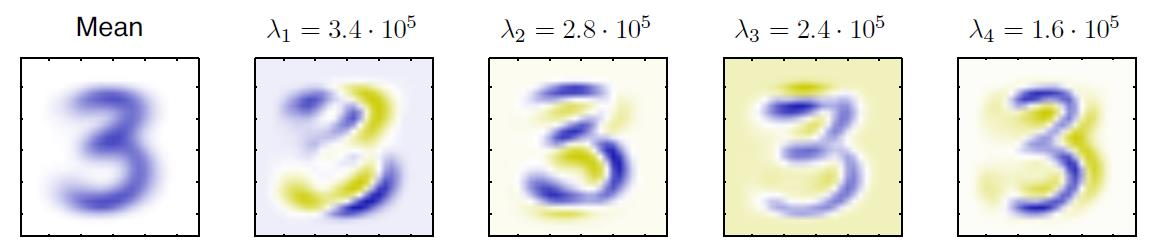
\includegraphics[width=10cm]{fig_2_1.jpg} 
    \caption{Digital number example of PCA}\label{fig_2_1}
\end{figure}
\begin{figure}[h] 
    \centering 
    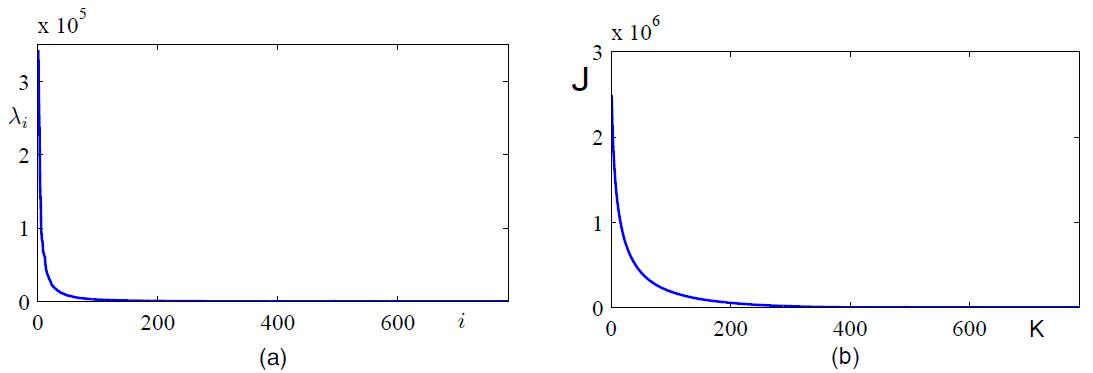
\includegraphics[width=10cm]{fig_2_2.jpg} 
    \caption{Eigenvalue spectrum example (left), and approximation error (right)}\label{fig_2_2}
\end{figure}
\par We can see that (Figure \ref{fig_2_1}) the first 4 principal eigenvectors have very clear interpretation. The first one mainly deals with tilting, and the 4th one probably handles scaling. Also the eigenvalues show the importance of each principal vector.
\par It's also very helpful to look at the eigenvalue spectrum (Figure \ref{fig_2_2}). For structured data like natural images, there is usually a fast decay in its eigenvalue spectrum. Since the reconstruction error depends on the sum of eigenvalues we ignore, there is usually a fast decay in reconstruction loss w.r.t. the number of principal components.
\par In the discussion so far, we always assume that the number of principal components (also for the reduced dimension number in Linear Autoencoder) is predefined and fixed. A natural question to ask is how should we choose this number, which is sometimes called \emph{intrinsic dimensionality} . A heuristic strategy is to look at the spectrum of eigenvalues and detect the "knee" or "elbow". However, in practice, there are usually more things like the limit of computational power or storage that determine how we choose the number of reduced dimensions.
\begin{figure}[h] 
    \centering 
    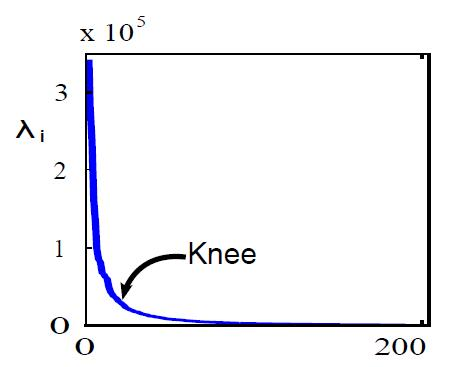
\includegraphics[width=6cm]{fig_2_3.jpg} 
    \caption{Detect "knee" to determine intrinsic dimensionality}\label{fig_2_3}
\end{figure}
\subsection{Comparison with Linear Autoencoder Network}
At this point, it is worth spending some time comparing the two dimension reduction method we learned:
\begin{itemize}
    \item PCA clarifies that one should (ideally) center the data, while it's not explicit in Linear Autoencoder.
    \item PCA representation is unique (if no eigenvalue multiplicities) and as such (in principle) interpretable.
    \item Linear autoencoder without weight sharing is highly non-interpretable (lack of identifiability).
    \item Linear autoencoder with weight sharing: ${\bf C=D^T}$ identifies the same subspace of $k$ principal eigenvectors (see discussion after Remark \ref{rmk_1_1}), but axes are non-identifiable. To modify an autoencoder to identify the principal axes, techniques like adding regularization to enforce ordering in the axis can be applied.
    \item General lesson for neural networks based method: caution with naively interpreting learned (neural) representations.
\end{itemize}
\par For the algorithm used to find the solution:
\begin{itemize}
    \item Compute one principal component at a time via power iterations: good for small $k$, conceptually easy and robust.
    \item Train a linear auto encoder via backpropagation: it's easily extensible and we use stochastic optimization (stochastic gradient descent), which is good for very large data set and has good convergence properties.
    \item Compute PCA from SVD: good for mid-sized problems, can leverage wealth of numerical techniques for SVD (e.g. QR decomposition)
\end{itemize}
\subsection{PCA via SVD}
The power iteration algorithm and eigen-decompostion, which has time complexity $O(m^3)$ for $\bm{\Sigma}\in\mathbb{R}^{m\times m}$, suffer from large $m$. A way to solve the problem for the case that $m$ is considerably large compared with $n$ is to use SVD, which only takes $O(mn^2)$ for ${\bf X}\in \mathbb{R}^{m\times n}$.
\par To compute the eigen-decomposition of ${\bf AA}^T$ via SVD:
\begin{equation*}
    {\bf AA}^T = ({\bf UDV})({\bf VD}^T{\bf U}^T) = {\bf UDI_nD}^T{\bf U}^T = {\bf U\Lambda U}^T
\end{equation*}
where ${\bf \Lambda} = {\bf DD}^T=\text{diag}(\lambda_1,\dots,\lambda_m)\in\mathbb{R}^{m\times m}$ and
\begin{equation*}
\lambda_i=\begin{cases}
\sigma_i^2& \text{for }1\leq i \leq \min\{n,m\}\\
0& \text{for }n< i \leq m
\end{cases}
\end{equation*}
Similarly we have ${\bf A}^T{\bf A}={\bf V\Lambda'V}^T$, where
\begin{equation*}
    {\bf \Lambda'} = {\bf D}^T{\bf D} = \text{diag}(\lambda'_1,\dots,\lambda'_n)\in\mathbb{R}^{n\times n},\ \lambda'_i=\begin{cases}
\lambda_i^2& \text{for }1\leq i \leq \min\{n,m\}\\
0& \text{for }m< i \leq n
\end{cases}
\end{equation*}
We see that ${\bf U}$, i.e. the left singular vectors of A, is the eigenvectors of ${\bf AA}^T$, and ${\bf V}$, i.e. the right singular vectors of A, is the eigenvectors of ${\bf A}^T{\bf A}$. ${\bf \Lambda}$ and ${\bf \Lambda}$ are identical up to zero padding. This shows that we can used the SVD of ${\bf X}$ to compute the eigen-decomposition of ${\bf \Sigma}=\frac{1}{n}{\bf XX}^T$. But when $n \gg m$, SVD is not so competitive. Also note that, eigen-decomposition of ${\bf \Sigma}$ suffers from very large and small $\sigma_i$'s in terms of numerical stability since it involves squares compared with using the SVD.

\end{document}
